% !TEX encoding = UTF-8 Unicode
% $Header: /cvsroot/latex-beamer/latex-beamer/solutions/conference-talks/conference-ornate-20min.en.tex,v 1.6 2004/10/07 20:53:08 tantau Exp $

\documentclass[handout]{beamer}
\usepackage{icomma}
\usepackage{xltxtra}
\newfontfamily\DejaSans{DejaVu Sans}

% This file is a solution template for:

% - Talk at a conference/colloquium.
% - Talk length is about 20min.
% - Style is ornate.

\mode<presentation>
{
  \usetheme{Warsaw}
  % or ...

  \setbeamercovered{transparent}
  % or whatever (possibly just delete it)
  
  \setbeamertemplate{navigation symbols}{}
  
  \newcommand*\oldmacro{}%
  \let\oldmacro\insertshorttitle%
  \renewcommand*\insertshorttitle{%
    \oldmacro\hfill%
    \insertframenumber\,/\,\inserttotalframenumber}
}

\usepackage[utf8]{inputenc}
% or whatever

\usepackage{times}
\usepackage{multirow}
\usepackage[T1]{fontenc}
\usepackage{graphicx}
\usepackage{eso-pic}
\usepackage{color}
\usepackage{tikz}
\usepackage{wasysym}
\usepackage{eurosym}

% Or whatever. Note that the encoding and the font should match. If T1
% does not look nice, try deleting the line with the fontenc.

\title[]
{Preference Elicitation in Mangaki:\\How Weird is Your Taste in Manga \& Anime?}

\author[]
{Jill-Jênn Vie}

\institute[]
{
\includegraphics[width=0.42\linewidth]{figures/mangaki.png}}

\date
{October 20, 2016}

\begin{document}

\definecolor{vert}{rgb}{0.07 0.54 0.07}

{
\setbeamertemplate{headline}[default]
\begin{frame}
	\titlepage
\end{frame}
}

\def\R{\mathcal{R}}
\def\N{N}
\newcommand\good{{\color{green!50!black}\DejaSans ☺}}
\newcommand\neutral{{\color{blue}\DejaSans 😐}}
\newcommand\bad{{\color{red}\DejaSans ☹}}

\begin{frame}
  \frametitle{France is the 2\textsuperscript{nd} manga consumer in the world}
  \begin{itemize}
    \item[1.] Japan - 500M volumes
    \item[2.] France - 13M volumes 
    \item[3.] US - 9M volumes
  \end{itemize}
  \pause
  \begin{exampleblock}{Japan Expo 2015, summer festival about Japanese culture}
  \begin{itemize}
  \item 250k tickets over 4 days
  \item \euro130 per person
  \item More than \euro8M every year
  \end{itemize}
  \end{exampleblock}
\end{frame}

\begin{frame}
  \frametitle{Mangaki}
  \begin{columns}
  \begin{column}{0.5\textwidth}
    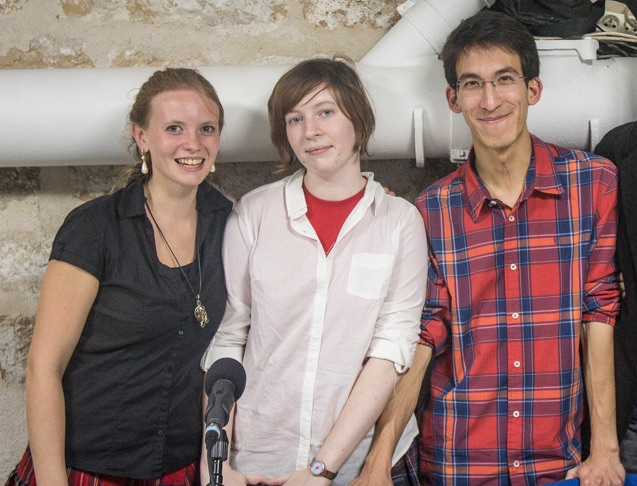
\includegraphics[width=\textwidth]{figures/trio.jpg}
  \end{column}
  \begin{column}{0.5\textwidth}
    {\em Let's use algorithms to discover pearls of Japanese culture!}\\[5mm]
    23 members:\\\hspace{7mm} 3 mad developers\\\hspace{14mm} 1 graphic designer\\\hspace{21mm} 2 interns
  \end{column}
  \end{columns}
  \vspace{2mm}
  \begin{itemize}
  \item Feb 2014 - PhD about Adaptive Testing
  \item Oct 2014 - \alert{Mangaki}
  \item Oct 2015 - Student Demo Cup winner, Microsoft Ventures prize
  \item Feb 2016 - Japanese Cultural Institute Prize, Paris\\[1mm]\pause\hfill\small\em We flew to Tokyo!
  \end{itemize}
\end{frame}

\newcommand\discrete[1]{\textcolor{gray}{\hfill {\em \small #1}}}

\begin{frame}
	\frametitle{Mangaki}
    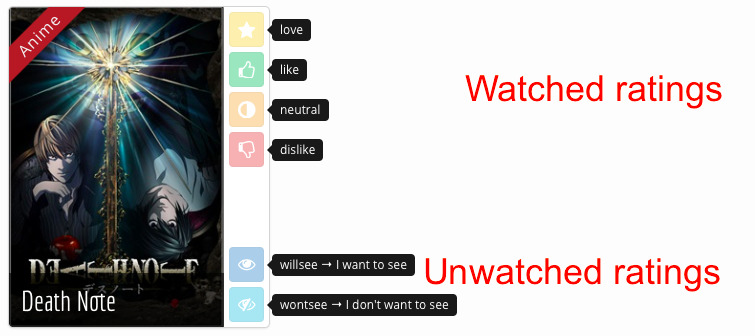
\includegraphics[width=\textwidth]{figures/ratings.jpg}
	\begin{itemize}
	\item 2100 users
	\item 150 $\rightarrow$ 15000 works \discrete{anime / manga / OST}
	\item 310000 ratings \discrete{fav / like / dislike / neutral / willsee / wontsee}
	\item People rate a few works \discrete{Preference Elicitation}
  \item And receive recommendations \discrete{Collaborative Filtering}
	\end{itemize}
\end{frame}

\begin{frame}
	\frametitle{Collaborative Filtering}
	\begin{block}{Problem}
		\begin{itemize}[<+->]
		\item Users $u = 1, \ldots, n$ and items $i = 1, \ldots, m$
		\item Every user $u$ rates some items $\R_u$\\(\alert{$r_{ui}$}: rating of user $u$ on item $i$)
        \item How to guess unknown ratings?
		\end{itemize}
	\end{block}
	\pause
	\begin{exampleblock}{$k$-nearest neighbor}
        \begin{itemize}
        \item Similarity score between users:
        \[ score(u, v) = \frac{\R_u \cdot \R_v}{||\R_u|| \cdot ||\R_v||}. \]
        \item Let us find the $k$ nearest neighbors of the user
        \item And recommend what they liked that he did not rate
        \end{itemize}
	\end{exampleblock}
\end{frame}

\begin{frame}
    \frametitle{Preference Elicitation}
    \begin{block}{Problem}
        What questions to ask adaptively to a new user?
    \end{block}
    \pause
    \begin{exampleblock}{4 decks}
        \begin{itemize}
        \item Popularity
        \item Controversy (Reddit)
        \[ controversy(L, D) = {(L + D)}^{min(L / D, D / L)} \]
        \item Most liked
        \item \emph{Precious pearls}: few rates but almost no dislike
        \end{itemize}
    \end{exampleblock}
    Problem: most people cannot rate the controversial items
\end{frame}

\begin{frame}
  \frametitle{Yahoo's Bootstrapping Decision Trees}
  \centering
  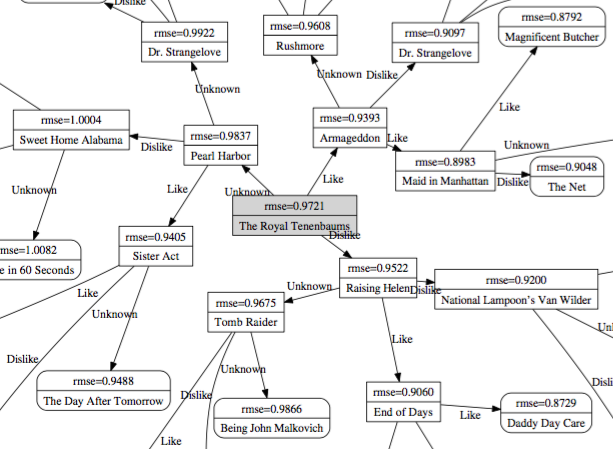
\includegraphics[width=0.9\linewidth]{figures/decisiontree.png}\\
  Good balance between like, dislike and unknown outcomes.
\end{frame}

\begin{frame}
	\frametitle{Matrix Completion}
	If the matrix of ratings is assumed \alert{low rank}:
	\[ M = \left(\begin{array}{c}
	\R_1\\
	\R_2\\
	\vdots\\
	\R_n
	\end{array}\right) = \raisebox{-1cm}{\begin{tikzpicture}
	\draw (0,0) rectangle (2.5,2);
	\end{tikzpicture}} =
	\raisebox{-1cm}{\begin{tikzpicture}
	\draw (0,0) rectangle ++(1,2);
	\draw node at (0.5,1) {$C$};
	\draw (1.1,1) rectangle ++(2.5,1);
	\draw node at (2.35,1.5) {$P$};
	\end{tikzpicture}} \]
	Every line $\R_u$ is a linear combination of few profiles $P$.
  \pause
  \begin{exampleblock}{1. Explicable profiles}
	\begin{tabular}{@{}lccc@{}}
	If $P$ & $P_1$ : adventure & $P_2$ : romance & $P_3$ : plot twist\\
	And $C_u$ & $0,2$ & $-0,5$ & $0,6$
	\end{tabular}\\
	$\Rightarrow$ $u$ \alert{likes a bit} adventure, \alert{dislikes} romance, \alert{loves} plot twists.
	\end{exampleblock}
  \pause
  \begin{exampleblock}{2. We get user2vec \& item2vec in the same space!}
  $\Rightarrow$ An user likes items that are \alert{in its direction}.\\[1pt]\vfill
  \end{exampleblock}
\end{frame}

\begin{frame}
    \frametitle{Mangaki's Explained Profiles}
    \begin{block}{$P_1$ loves Ghibli and cyberpunk, hates teen stories}
    \begin{itemize}
    \item[\good] \emph{Princess Mononoké}, \emph{Spirited Away} (Chihiro)
    \item[\good] \emph{Cowboy Bebop}, space opera similar to \emph{Firefly}
    \item[\good] \emph{Paprika}, which inspired \emph{Inception}
    \item[\bad] \emph{Naruto}, \emph{Bleach}
    \end{itemize}
    \end{block}
    \pause
    \begin{block}{$P_2$ lives really weird works, hates the most popular works}
    \begin{itemize}
    \item[\good] Erotic stories
    \item[\good] Same-family homosexual romances:\\\emph{Kiss x Sis}, \emph{Papa to Kiss in the Dark}
    \item[\bad] \emph{Attack on Titan}, \emph{Death Note}
    \end{itemize}
    \end{block}
\end{frame}

\begin{frame}
	\frametitle{user2vec: plotting every user on a map}
	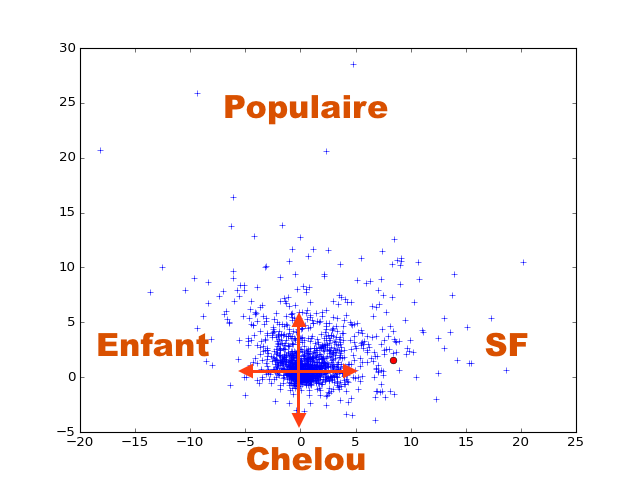
\includegraphics[width=\linewidth]{figures/map.png}
\end{frame}

\begin{frame}
	\frametitle{user2vec: plotting every user on a map}
	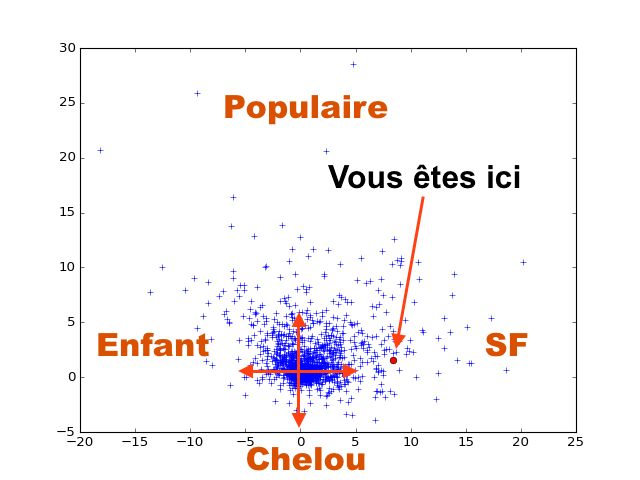
\includegraphics[width=\linewidth]{figures/here.png}
\end{frame}

\begin{frame}
  \frametitle{What questions should be asked?}
  \centering
  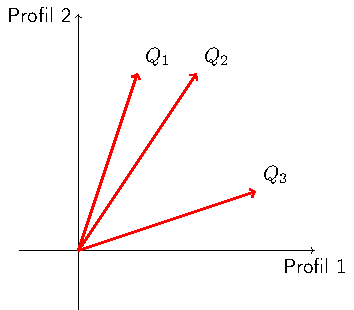
\includegraphics[]{figures/vectors.pdf}
\end{frame}

\begin{frame}
    \frametitle{Link with diversity}
    \centering
    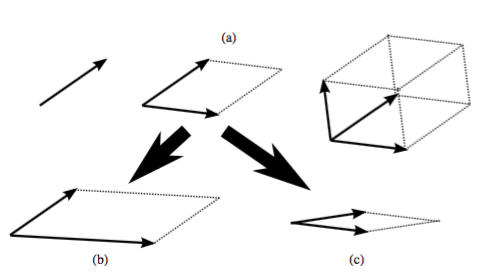
\includegraphics[width=0.7\linewidth]{figures/vol.png}
    \begin{itemize}
    \item The determinant is the square of the volume of the vectors
    \item Non-correlated (\alert{diverse}) vectors will increase the volume
    \item We need to sample $k$ diverse elements efficiently
    \end{itemize}
\end{frame}

\begin{frame}
    \frametitle{Modelling Diversity: Determinantal Point Processes}
    Let's sample a few items that are \alert{far from each other} and ask them to the user.
    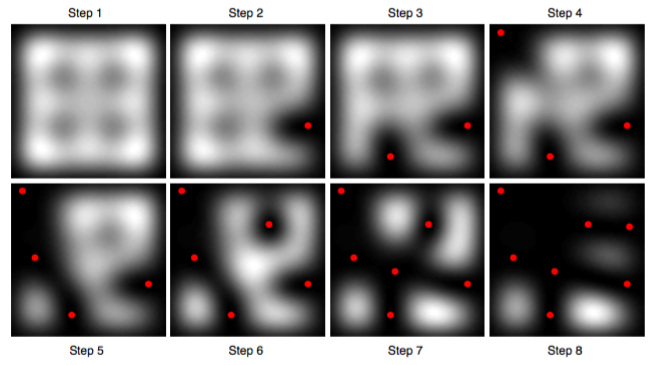
\includegraphics[width=\linewidth]{figures/dpp.png}
\end{frame}

\begin{frame}
    \frametitle{Determinantal Point Processes}
    We want to sample over $n$ items\\
    $K : n \times n$ \alert{similarity matrix} over items (positive semidefinite)\\[5mm]
    $P$ is a \alert{determinantal point process} if $Y$ is drawn such that:
    \[ \forall A \subset Y, \quad P(A \subseteq Y) \propto det(K_A) = Vol(\{x_i\}_{i \in A})^2 \]
    \begin{example}
    \begin{columns}
    \begin{column}{0.5\textwidth}
    \[ K = \left(\begin{array}{cccc}
    1 & 2 & 3 & 4\\
    2 & 5 & 6 & 7\\
    3 & 6 & 8 & 9\\
    4 & 7 & 9 & 0
    \end{array}\right) \]
    \end{column}
    \begin{column}{0.5\textwidth}
    $A = \{1, 2, 4\}$ will be included with probability prop. to
    \[ K_A = det\left(\begin{array}{ccc}
    1 & 2 & 4\\
    2 & 5 & 7\\
    4 & 7 & 0
    \end{array}\right) \]
    \end{column}
    \end{columns}
    \end{example}
\end{frame}

\begin{frame}
  \frametitle{Results}
  We assume the eigenvalues of $K$ are known.
  \begin{block}{Kulesza \& Taskar, ICML 2011}
  Sampling $k$ diverse elements from a DPP of size $n$ has complexity $O(nk^2)$.
  \end{block}
  \pause
  \begin{block}{Kang (Samsung), NIPS 2013}
  We found an algorithm $\epsilon$-close with complexity $O(k^3 \log (k / \epsilon))$.
  \end{block}
  \pause
  \begin{block}{Rebeschini \& Karbasi, COLT 2015}
  No, you did not.\\\pause
  Your proof of complexity is false, but at least your algorithm samples correctly.
  \end{block}
\end{frame}

\begin{frame}
  \frametitle{Work in progress: Preference Elicitation in Mangaki}
  \begin{itemize}
  \item Keep the 100 most popular works
  \item Pick 5 diverse works using $k$-DPP
  \item Ask the user to rate them
  \item Estimate the user's vector
  \item Filter less informative works accordingly
  \item Repeat.
  \end{itemize}
\end{frame}

\begin{frame}
  \frametitle{Preference elicitation: sampling a diverse subset}
  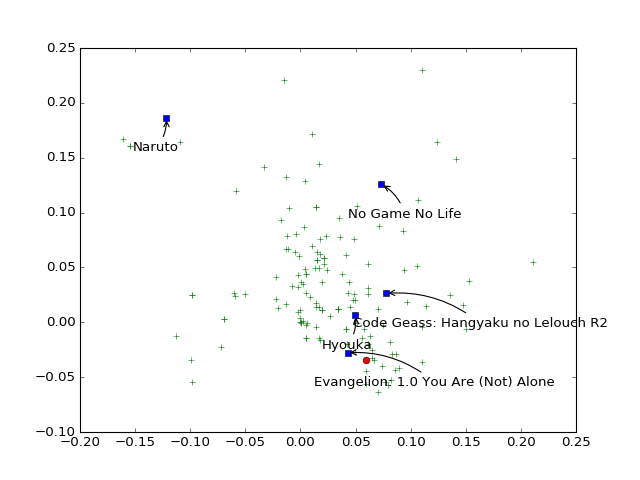
\includegraphics[width=\linewidth]{figures/1.png}
\end{frame}

\begin{frame}
  \frametitle{Summing up}
  \begin{itemize}
    \item We get a nice subset of $k$ questions over $n$ in $O(nk^3)$
    \item (after preprocessing $O(n^3)$)
    \item Not the best subset (NP-hard), but a nice subset
    \item Good way not to ask the same questions to everyone
  \end{itemize}
\end{frame}

\begin{frame}
	\frametitle{Thanks for listening!}
  \LARGE
	\begin{columns}
	\begin{column}{0.5\textwidth}
  
\includegraphics[width=1cm]{figures/twitter.png}\,\,\raisebox{1.5mm}{@MangakiFR}\\[1mm]
  research.mangaki.fr
	\end{column}
	\begin{column}{0.5\textwidth}
	\centering
  \huge We're on GitHub!
  \end{column}
  \end{columns}
  \vspace{5mm}
  
\includegraphics[width=\linewidth]{figures/mangaki.png}
\end{frame}


	% \small (P. S. -- C'est la Code Week, apprenez à coder et tentez le concours \alert{figures/Prologin.org}, c'est gratuit et sans obligation d'achat !)

\end{document}